\centering [\textit{Teil 3}]
\pend
\pstart
%\vspace*{0,5em}
\noindent
Supersunt non paucae circa motum et mechanicae difficultates penitius rimandae,
e.g. ortum est eo majore opus esse vi\protect\index{Sachverzeichnis}{vis},
quo altius facit ascendere corpus datum eodem
\edtext{tempore seu primo momento, cum tamen}{\lemma{tempore}\Bfootnote{\textit{(1)}\ . Cum tamen \textit{(2)}\ seu [...] tamen \textit{L}}}
ea vis quae corpus ascendere facit,
confligat cum illo liquido sive vento cujus motus est causa descensus gravium\protect\index{Sachverzeichnis}{grave},
et quidem diutius cum eo confligat quo tardius movetur.
Jam temporis non loci magnitudine aestimandas esse retardationes patet ex gravium,
ut pendulorum\protect\index{Sachverzeichnis}{pendulum} ascensu post descensum.
\pend
\pstart
Experimento primum opus est, an majori vi opus sit, ad efficiendum ut corpus aliquod moveatur contra ventum celerius quam tardius.
Si exiguo tempore plurimum spatii percurrit, videtur exiguo tempore plurimum venti experiri, ut qui adverso flumine natat.
Ictus\protect\index{Sachverzeichnis}{ictus} ergo non temporum momentis, sed spatii punctis aestimandi sunt.
At qui fit ut in descensu gravium ictus quovis temporis momento repetiti intelligantur.
Forte ergo contrarium verum est.
\pend
\pstart
 \noindent
\begin{minipage}[t]{0.53\textwidth}
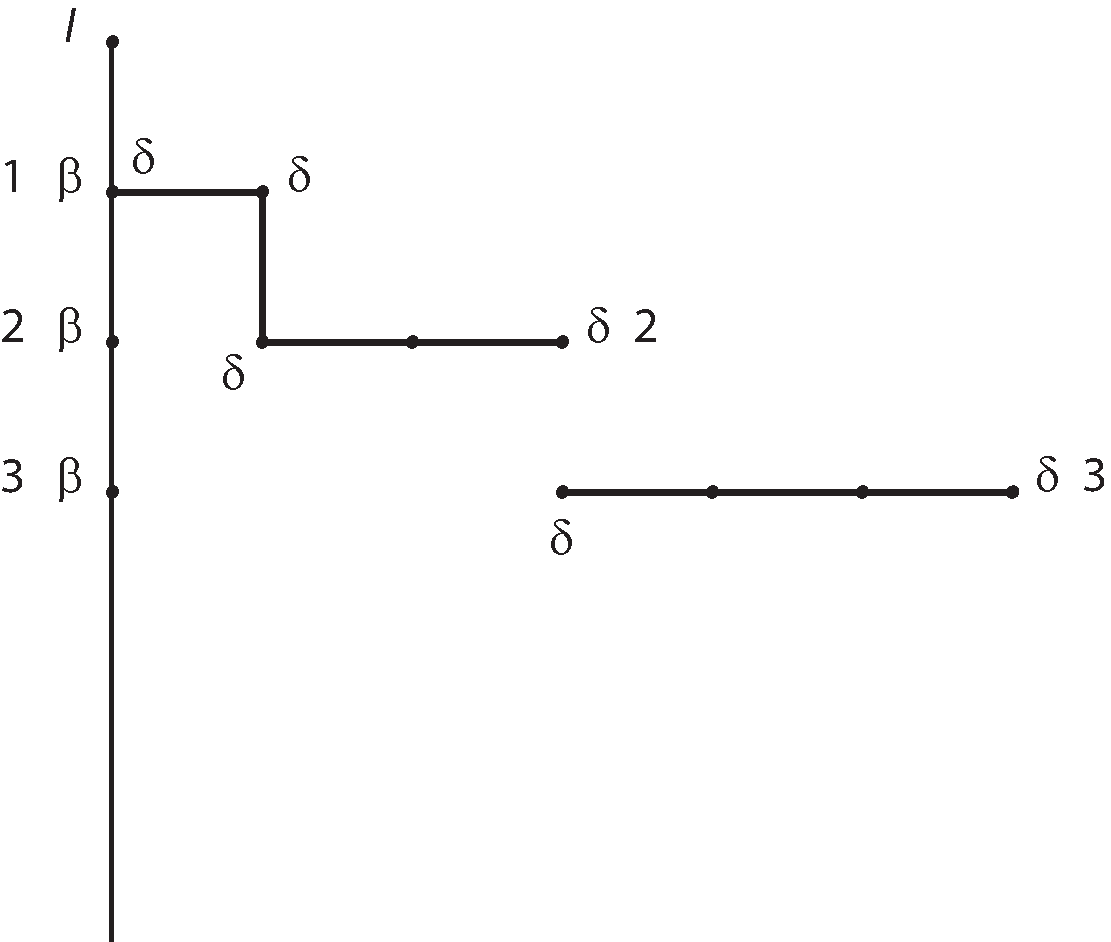
\includegraphics[trim = 0mm -5mm 0mm 0mm, clip, width=0.98\textwidth]{images/lh0350911_007v-d1.pdf}
\end{minipage}
\hspace*{13,3mm}
\begin{minipage}[t]{0.47\textwidth}
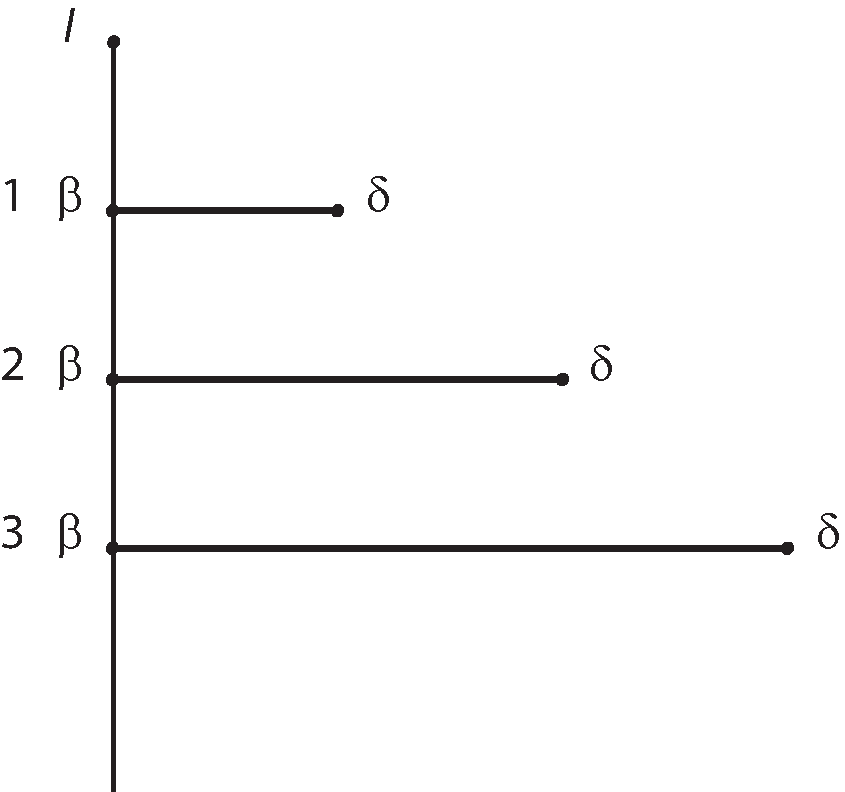
\includegraphics[trim = 0mm -5mm 0mm 0mm, clip, width=0.8\textwidth]{images/lh0350911_007v-d2.pdf}
\end{minipage}
\hspace*{22mm} [\textit{Fig. 4, gestrichen}]\hspace{54mm} [\textit{Fig. 5}]
\pend
\vspace{1em}
\count\Bfootins=1200
\count\Afootins=1200
\pstart
 Si $\displaystyle \beta\beta$ sint \setline{1}spatia aequalia,
ponendo eodem spatio percurso\protect\index{Sachverzeichnis}{spatium percursum}
[eundem impetum\protect\index{Sachverzeichnis}{impetus}]\edtext{}{\Bfootnote{idem impetus\textit{\ L \"{a}ndert Hrsg.}}}
acquiri, erit primo spatio $\displaystyle \beta\beta$,
\edtext{seu $\displaystyle \mathrm{I}\beta$}{\lemma{seu}\Bfootnote{\textit{(1)}\ $\displaystyle \beta\beta$ \textit{(2)}\ $\displaystyle \mathrm{I}\beta$ \textit{L}}}
percurso celeritas
\edtext{quaesita $\displaystyle 1\,\beta\delta,$ 2\textsuperscript{do} $\displaystyle \beta\beta$}{\lemma{quaesita}\Bfootnote{%
\textit{(1)}\ $\displaystyle 1\,\delta\delta$ %
\textit{(2)}\ $\displaystyle 1\,\beta\delta,$ %
\textit{(a)}\ secundo $\displaystyle \beta$ %
\textit{(b)}\ 2\textsuperscript{do} $\displaystyle \beta\beta$ \textit{L}}}
percurso \edtext{erit impetus}{\lemma{erit}\Bfootnote{\textit{(1)}\ celeritas \textit{(2)}\ impetus \textit{L}}} quaesitus \edtext{$\displaystyle 2\,\beta\delta$}{\lemma{quaesitus}\Bfootnote{\textit{(1)}\ $\displaystyle 2\,\delta\delta$ \textit{(2)}\ $\displaystyle 2\,\beta\delta$ \textit{L}}}, tertio spatio percurso  erunt impetus quaesiti \edtext{$\displaystyle 3\,\beta\delta$}{\lemma{quaesiti}\Bfootnote{\textit{(1)}\ $\displaystyle 3\,\delta\delta$ \textit{(2)}\ $\displaystyle 3\,\beta\delta$ \textit{L}}}. Erunt ergo impetus quaesiti spatiis percursis reciproce
proportionales et ideo impetus quaesiti exhibebuntur applicatis trianguli.
Sive impetus quaesiti erunt spatiis percursis proportionales.
\edtext{Ergo momenta quibus quodlibet spatii punctum percurritur, erunt spatiis reciproce percursis}{\lemma{Ergo}\Bfootnote{\textit{(1)}\ tempus \textit{(2)}\ temporum decrementa erunt spatiis percursis \textit{ (3) }\ momenta [...] percursis \textit{L}}}
proportionalia. Ergo
\edtext{si spatia percursa sint ut numeri}{\lemma{si}\Bfootnote{\textit{(1)}\ tempora sint ut numeri \textit{(2)}\ spatia [...] numeri, \textit{L}}},
tempora\protect\index{Sachverzeichnis}{tempus} erunt ut logarithmi. Ergo
si tempora sint proportionis
\edtext{Arithmeticae spatia}{\lemma{Arithmeticae}\Bfootnote{\textit{(1)}\ tempora \textit{(2)}\ spatia \textit{L}}}
sint proportionis Geometricae. Contrarium est in motu frictionis.
Itaque si corpus tempore ut 1. descendat per
\edtext{altitudinem pedum 10.}{\lemma{altitudinem}\Bfootnote{\textit{(1)}\ ut ab in \textit{(2)}\ pedum 10. \textit{L}}}
id tempore \edtext{ut 10}{\lemma{ut}\Bfootnote{\textit{(1)}\ 4 \textit{(2)}\ 10 \textit{L}}}
descendet per \edtext{altitudinem pedum 10000000000}{\lemma{altitudinem pedum}\Bfootnote{\textit{(1)}\ 81 \textit{(2)}\ 10,000 \textit{(3)}\ 10000000000 \textit{L}}}
quod tamen experientiae repugnat, itaque \edtext{[non]}{\lemma{non}\Bfootnote{\textit{erg. Hrsg.}}}
sequitur.
Nempe si numerus pedum sit $\displaystyle b$. unitas sit 1.
tunc si tempore ut 1 ascendat per numerum pedum: $\displaystyle ba^9$,
tempore ut 10 ascendet per numerum pedum $\displaystyle b^{10}$.
Nam si tempore \edtext{ut 1}{\lemma{ut}\Bfootnote{\textit{(1)}\ $\displaystyle b$ \textit{(2)}\ 1 \textit{L}}}
ascendat per altitudinem pedum $\displaystyle ba$, tempore ut 2 ascendet per altitudinem
\edtext{pedum: $\displaystyle b^2$}{\lemma{pedum:}\Bfootnote{\textit{(1)}\ $\displaystyle ba$ \textit{(2)}\ $\displaystyle b^2$ \textit{L}}}
erunt ergo ut \edtext{1 ad $\displaystyle \frac{b}{a}$. seu ut $\displaystyle \frac{b}{a}$ ad $\displaystyle \frac{b^2}{a^2}$}{\lemma{ad $\displaystyle \frac{b}{a}$.}\Bfootnote{\textit{(1)}\ sed hoc esse non debet, debent enim esse, ut \textit{(2)}\ seu [...] $\displaystyle \frac{b^2}{a^2}$. \textit{L}}}.
\rule[-4mm]{0mm}{10mm}Cum ergo haec videantur experientiae repugnare, crediderim
\edtext{hypothesin Galilaei\protect\index{Namensregister}{\textso{Galilei} (Galilaeus, Galileus), Galileo 1564-1642}}{\lemma{hypothesin Galilaei}\Cfootnote{Galilei nimmt tats\"{a}chlich an, dass bei einer gleichm\"{a}{\ss}ig beschleunigten Bewegung (wie etwa beim Fall schwerer K\"{o}rper) die Geschwindigkeit gem\"{a}{\ss} der Zeit, nicht gem\"{a}{\ss} dem Raum w\"{a}chst. Siehe \cite{00050}\cite{00048}\textit{Discorsi}, Leiden 1638, S. 157f. und 163-165 (\textit{GO} VIII, S. 197f. und 202-204).}}
esse veriorem. Imo videtur magnus ille numerus non sequi, sed opus esse duobus experimentis,\edtext{}{\lemma{}\Afootnote{\textit{Am Rand:} NB\vspace{-6mm}}}
nempe ex tanto tempore labitur per spatium tantum alio tempore versus per aliud spatium tantum;
inter haec duo spatia quaerantur continue proportionales mediae, vel etiam tertiae, et ita
res determinari poterit.
Ecce ergo dubitationem de applicatione demonstrationum
Galilaei\protect\index{Namensregister}{\textso{Galilei} (Galilaeus, Galileus), Galileo 1564-1642}
de motu uniformiter accelerato\protect\index{Sachverzeichnis}{motus uniformiter acceleratus} ad motum gravium.%\pend